\documentclass[journal]{IEEEtran}
\usepackage{cite}
\usepackage{amsmath,amssymb,amsfonts}
\usepackage{graphicx,booktabs,array,tabularx,multirow}
\usepackage{xcolor,url}
\usepackage{algorithm,algorithmic}
\usepackage{tikz}
\usetikzlibrary{arrows.meta,positioning,calc,fit,backgrounds,shapes.geometric}
\usepackage[hidelinks]{hyperref}
\newcolumntype{Y}{>{\raggedright\arraybackslash}X}
\newcommand{\etal}{\textit{et al.}}
\newcommand{\code}[1]{\texttt{#1}}
\renewcommand{\topfraction}{0.9}
\renewcommand{\dbltopfraction}{0.9}
\renewcommand{\textfraction}{0.08}
\setcounter{topnumber}{3}
\setcounter{dbltopnumber}{2}
\setcounter{totalnumber}{5}
\title{Frame-Coherent Gravity-Locked EO/IR Panorama Stabilization: Fixed-Point Algorithms and FPGA Architecture}
\author{Muhammad~Awais and Youngbae~Hwang%
\thanks{Corresponding author: Youngbae Hwang.}%
\thanks{M.~Awais is with the Department of Intelligent Systems and Robotics, Chungbuk National University, Cheongju 28644, Republic of Korea (e-mail: auuais@live.com).}%
\thanks{Y.~Hwang is with the Department of Electronics Engineering, College of Electrical and Computer Engineering, Chungbuk National University, Cheongju 28644, Republic of Korea (e-mail: ybhwang@cbnu.ac.kr).}}
\markboth{Manuscript for IEEE Transactions on Circuits and Systems for Video Technology}{Awais and Hwang: Frame-Coherent Gravity-Locked Panorama Stabilization}
\begin{document}
\maketitle
\begin{abstract}
Gravity-referenced stabilization of a multi-camera panorama requires azimuth-dependent correction and consistent association between images and inertial pose. We present a fixed-point EO/IR algorithm and FPGA architecture that retain calibrated cylindrical maps while deriving camera-specific roll and pitch from rig pose and mounting angles. Separate EO/IR histories associate pose snapshots with leased source framesets; coefficients remain frozen through table construction and rendering. The data path uses DDR capture/replay, a three-row source ring, and bounded output-row storage. Validation separates numerical correctness, implementation feasibility, and physical observations: 1,342 camera-projection vectors match the compiled C reference, six-camera control passes 266 cases, and each of two renderer suites matches 14,112,000 reference pixels. Reanalysis of archived software videos gives marker-orientation standard deviations of $7.410^\circ$, $1.177^\circ$, and $7.079^\circ$ for raw, inertially corrected, and rigid-flow outputs on 448 common frames. Saved stitching comparisons retain matched identities and failures. Routed timing, historical pipeline measurements, and camera raster/content-rate tests are reported with their configurations and event boundaries. The evidence supports a reproducible implementation and configuration-specific observations; independent current-hardware dynamic leveling accuracy, exposure-time alignment, and sustained throughput remain qualification limits.
\end{abstract}
\begin{IEEEkeywords}
Panoramic imaging, inertial stabilization, FPGA, fixed-point arithmetic, frame synchronization, infrared imaging, hardware verification.
\end{IEEEkeywords}

\section{Introduction}
\IEEEPARstart{A}{ rigid} multi-camera rig can provide continuous panoramic coverage without mechanical scanning. In electro-optical (EO) and infrared (IR) systems, roll and pitch perturb the viewing direction differently at each camera azimuth. Independently correcting a completed panorama with a planar transform does not, in general, reproduce a calibrated pre-stitch correction. However, geometric expressiveness is only part of the implementation problem. When camera capture, external memory, inertial updates, and output scanout run asynchronously, applying a correct transform to the wrong source frame produces a wrong result.

This work addresses that joint numerical and temporal problem. The target is a calibrated six-view cylindrical renderer with a low-dimensional gravity correction. The algorithm projects two live rig angles through six fixed camera mounts. The hardware then associates the resulting correction with the selected source frameset and retains it throughout the rendering pass. This association is especially important when a completed source frame waits in memory: the most recently received pose at render start need not describe that frame. A second source of ambiguity arises when EO and IR counters have the same numeric value but refer to unrelated trigger events.

The architecture therefore distinguishes \emph{pose receipt}, \emph{trigger association}, \emph{source selection}, and \emph{output publication}. These events cannot be collapsed into one frame-rate or latency number. The implementation also preserves the known optical maps while introducing the C camera-angle computation. Numerical equivalence at the angle interface is tested independently of equivalence to the preserved pixel mapper; the newer C application's optical parameters are not silently substituted into the hardware.

The contributions are:
\begin{enumerate}
\item A specified fixed-point camera-angle transformation, including rotation order, lookup precision, signed rounding, one-pass global limiting, mounting parameters, and the separate renderer range limit.
\item A frame-coherent hardware contract with independent EO/IR pose histories, exact epoch lookup, calibration-version checks, static fallback, and coefficient freezing across table construction and source replay.
\item A reproducible study separating C/RTL regression, routed resource/timing results, historical pipeline observations, and camera raster/content synchronization. Archived software comparisons use matched case/pair identities for static alignment and common detected marker/frame identities for orientation steadiness.
\end{enumerate}

The study does not treat scene-independent inertial input as an independent measurement of leveling accuracy, nor equate a routed design with measured system throughput. Quantitative hardware claims below are tied to archived measurements with identified configurations.

\section{Related Work and Scope}
\label{sec:related}
Visual stabilization estimates image motion and then smooths a camera path or a spatially varying field. Bundled Camera Paths and MeshFlow demonstrate different tradeoffs between local motion representation, optimization, and online latency \cite{liu2013bundled,liu2016meshflow}. These methods can accommodate effects beyond a two-angle model, including parallax and nonrigid residuals, at the cost of image-based estimation. Their accuracy depends on scene content and their memory/compute requirements depend on the implementation; they are not categorically incompatible with hardware.

Inertial stabilization avoids image matching for rotational motion. Karpenko \etal\ use gyroscopes for stabilization and rolling-shutter correction \cite{karpenko2011gyro}. Fused approaches combine inertial and visual information rather than treating them as exclusive alternatives \cite{shi2022deepfvs}. The present system uses an upstream attitude estimate but concentrates on camera projection, transport coherence, and renderer scheduling. It neither introduces a new attitude filter nor demonstrates that one filter dominates another on independent ground truth.

Omnidirectional stabilization can model nonlinear motion on a sphere or a cylinder; Kopf's 360-degree formulation is an example \cite{kopf2016omnistab}. Thus, an azimuth-dependent horizon error is not intrinsically uncorrectable after stitching. Pre-stitch correction is chosen here because source validity, camera overlap, and the existing calibrated mapper are available before blending. The relevant comparison is between specific motion models and sampling orders, not between all pre- and post-stitch methods.

For mobile multi-camera panoramas, Hamza \etal\ combine global motion correction, camera-region correction weighted by blend masks, and local geometric warping \cite{hamza2015panovideo}. Their image-based formulation explicitly handles inter-camera jitter. The present rigid-rig model instead derives camera corrections from one roll/pitch estimate and addresses their fixed-point implementation and source-frame association; it does not estimate independent camera vibration.

Image stitching likewise spans calibrated maps, projective registration, and learned warps. Brown and Lowe establish a feature-based panoramic formulation \cite{brown2007panorama}; UDIS++ addresses parallax in unsupervised image stitching \cite{nie2023parallax}; StabStitch++ addresses temporal warping shake in online video stitching \cite{nie2025stabstitch2}. Their tasks differ from gravity leveling. Our saved-output comparison tests alignment on one calibrated rig, with unequal preprocessing and adaptation policies explicitly recorded. It does not establish state-of-the-art performance across datasets or an infrared generalization advantage over unevaluated methods.

Fixed-transform hardware stitching demonstrates the efficiency of exploiting a known camera arrangement \cite{suk2015hwstitch}. We extend that design setting with pose-dependent coefficients and a source/pose association contract. The implemented system uses external frame storage, replay arbitration, source rings, and output buffering. Those costs are included in the resource and bandwidth discussion.

\section{Geometry, Timing, and Evaluation Definitions}
\label{sec:problem}
\subsection{Gravity Referencing on a Cylinder}
For geometric motivation, let a cylindrical viewing ray be proportional to
$\mathbf d(\vartheta,v)=[\sin\vartheta,\ v/f_c,\ \cos\vartheta]^\top$, where the second axis is vertical, $f_c$ is the cylindrical focal parameter, and $v$ is measured from the nominal horizon. If $\mathbf g=[g_x,g_y,g_z]^\top$ is gravity expressed in this coordinate system, a horizontal scene direction satisfies $\mathbf g^\top\mathbf d=0$. For $g_y\ne0$, its horizon is
\begin{equation}
 v_h(\vartheta)=-f_c\frac{g_x\sin\vartheta+g_z\cos\vartheta}{g_y}.
 \label{eq:cylhorizon}
\end{equation}
A small rig tilt therefore creates an approximately sinusoidal vertical deviation across azimuth. In a camera-centered approximation, the same tilt produces different local roll and pitch at different mount yaw angles. Per-camera pre-alignment is a compact way to represent this dependence before calibrated projection and blending. The code-level axis and multiplication conventions are specified separately in Section~\ref{sec:algorithm}; physical sensor-axis signs must be verified on the rig.

Equation~\eqref{eq:cylhorizon} also identifies a limitation of a planar baseline: a correction $a\vartheta+b$ cannot in general cancel the sinusoid across a wide field. It does \emph{not} prove that a general global image warp cannot correct it. A suitable spherical rotation or nonlinear cylindrical warp can represent that transformation. Moreover, a single-depth rotational model cannot remove translation-induced parallax, rolling-shutter effects, or unequal exposure times.

\subsection{Three Consistency Requirements}
Let $F_{s,e}$ denote a complete source frameset of sensor family $s\in\{\mathrm{EO},\mathrm{IR}\}$ and trigger-association tag $e$. Let $P_{s,e}$ be the stored pose/control snapshot and $C_j$ the mounting calibration at revision $j$. A valid rendering pass requires:
\begin{enumerate}
\item \emph{Numerical consistency}: the projection and pixel mapper use their documented units, quantizers, angle ranges, and optical profile.
\item \emph{State consistency}: the pass uses one accepted $(F_{s,e},P_{s,e},C_j)$ association; changing input registers cannot change a partly built table or an active frame.
\item \emph{Physical temporal consistency}: the pose represents the actual camera exposure interval, to the accuracy required by the motion.
\end{enumerate}
The first two properties can be checked against source and RTL tests. The third requires a measurement of camera/ISP delay, attitude-estimator delay, transport timing, and exposure timing. Matching trigger tags establishes an association rule, not an exposure timestamp.

\subsection{Rates and Latency Boundaries}
A raster start counts an interface timing event. A distinct-frame estimate counts accepted content changes under a stated measurement rule. An output commit counts completion of a buffered image. These rates may differ because a camera repeats images, a renderer skips source epochs, or a display repeats its current buffer. A format label such as 1080p60 is therefore not a measurement of 60 independently exposed images/s.

For a trace with valid event associations, define descriptor-to-copy and descriptor-to-commit intervals as
\begin{equation}
 L_{dc}=t_{\rm copy\ done}-t_{\rm descriptor},\qquad
 L_{dp}=t_{\rm commit}-t_{\rm descriptor}.
 \label{eq:latencybounds}
\end{equation}
Neither includes sensor integration or ISP delay before the descriptor, and neither automatically includes display scanout. If the descriptor timestamp belongs to a newer frame than the consumed lease, these differences are diagnostics rather than the latency of that consumed frame. This caveat is applied to the archived measurements in Section~\ref{sec:hardware}.

For future dynamic tests, a horizon profile can be summarized by a detrended residual
\begin{equation}
 D_h=\sqrt{\frac{1}{|\Omega|}\sum_{x\in\Omega}
 [y_h(x)-(\hat a x+\hat b)]^2},
 \label{eq:dhr}
\end{equation}
where $(\hat a,\hat b)$ minimize squared error on a fixed valid support $\Omega$. This statistic removes an additive linear component on that support only. It is not invariant to arbitrary warps or changing crops. A horizon synthesized from the same IMU estimate that drives correction measures model consistency; an independent target or orientation instrument is required to measure physical leveling accuracy.

% Replacement algorithm and FPGA architecture sections.
% Required packages: amsmath, amssymb, graphicx, booktabs, tikz.
% Required TikZ libraries: arrows.meta, positioning, calc.
% Compile from the manuscript directory so figures/ resolves correctly.
% This file makes no claim of measured physical stabilization or throughput.

\section{Gravity-Referenced Camera Correction}
\label{sec:gl_algorithm}
\label{sec:algorithm}

\subsection{Scope and Calibration Contract}
The method separates static optical mapping, time-varying camera orientation,
and frame association. An archived inverse map accounts for the fixed lens,
cylindrical projection, crop, and strip placement. A low-rate orientation
engine converts one rig roll/pitch pair into six camera-specific corrections.
The renderer applies these corrections to the map segments associated with
one leased source frameset. The FPGA receives orientation estimates; it does
not estimate attitude from raw inertial samples. There is no live yaw input,
heading lock, translation estimate, or rolling-shutter model in this path.

For pure rotation and a calibrated central camera, a rotation in ray space
can be mapped back to a cylinder. Thus a sufficiently general global
spherical or cylindrical warp can compensate rotation. The practical issue
here is narrower: a common vertical shift or planar roll applied to an
already assembled panorama does not generally reproduce the different local
corrections around the ring. The proposed implementation uses camera-specific
affine corrections to retain the existing segment-based mapping and sampling
hardware. It is an approximation to ray reprojection, rather than a claim
that all global rotational correction is impossible.

Let camera $i$ have mounting yaw $\psi_i$, pitch $p_i^0$, and roll $r_i^0$.
The six EO yaws are $(0,60,120,180,240,300)^\circ$; the IR yaws are
$(90,150,210,270,330,390)^\circ$. The $390^\circ$ value is retained in
calibration and normalized modulo $360^\circ$ for trigonometric lookup.
Initial mounting roll and pitch are zero for all cameras. Subsequently,
per-camera UI roll/pitch trims are retained across boots. The MCU applies
the selected mounting profile once, recording revision \texttt{0x7106B1F1}
in a CRC-protected two-page journal. Runtime yaw edits are stored by the MCU,
but the present FPGA uses the fixed yaw constants above. Only roll/pitch
trims feed its orientation engine.

Table~\ref{tab:gl_calibration} distinguishes the installed optical profile
from the selected mounting-profile INI. In particular, adopting the mounting
angles does not regenerate the optical maps. The INI's example live poses
$(0.75,-5.00)^\circ$ for EO and $(1.25,6.50)^\circ$ for IR are test inputs,
not runtime defaults. Likewise its output-mode and DDR-offset fields are
not the hardware mode/address contract.

\begin{table*}[t]
\caption{Calibration and preserved optical configuration. The ``selected INI''
column is recorded for reproducibility; only its mounting arrays are imported.
Focal lengths and principal points are in original source pixels.}
\label{tab:gl_calibration}
\centering\footnotesize\setlength{\tabcolsep}{4.3pt}
\begin{tabular}{@{}lccc@{}}
\toprule
Parameter & Installed EO & Installed IR & Selected INI: EO / IR \\
\midrule
Source size; cameras & $1920\!\times\!1080$; 6 & $640\!\times\!512$; 6 & unchanged \\
$(f_x,f_y)$ & $(1141.834740,1142.434960)$ & $(564.835060,564.024805)$ & unchanged \\
Normalized principal point & $(0.489836,0.514300)$ & $(0.497330,0.476162)$ & unchanged \\
Distortion principal point & $(940.486,555.444)$ & $(318.291416,243.794865)$ & unchanged \\
$(k_1,k_2,k_3)$ & $(-.163318,.165940,-.064582)$ & $(-.327245098,.299803510,-.197210469)$ & unchanged \\
$(p_1,p_2)$ & $(.000236,.000773)$ & $(.000324600,.000015975)$ & unchanged \\
Map resize factor & $0.5$ & $1.0$ & $0.56296$ / $1.0$ \\
Cylindrical horizontal/vertical FOV & $57.56^\circ/48.56^\circ$ & $54.5^\circ/45.0^\circ$ & $77^\circ/54^\circ$ / $65^\circ/52^\circ$ \\
Crop height/width scale & $0.888/1.0$ & $0.9375/1.0$ & $0.79/0.70$ / $0.65/0.9$ \\
Map-profile overlap; feather strength & $50$; $1.0$ & $30$; $1.0$ & $60$; $1.0$ / $30$; $1.0$ \\
Logical panorama size & $3840\!\times\!480$ & $3576\!\times\!480$ & $3840\!\times\!480$ / $3240\!\times\!480$ \\
Source pitch shift, pixels/degree & $-9.80$ & $-8.72$ & newer C: $-17.408$ / $-8.72$ \\
Per-camera strip widths & $650,655,655,655,655,655$ & $616,621,640,621,621,621$ & installed segment ROMs retained \\
Panorama strip starts & $0,633,1271,1909,2547,3185$ & $0,587,1179,1771,2363,2955$ & installed placement retained \\
\bottomrule
\end{tabular}
\end{table*}

\subsection{Upstream Attitude Estimate}
The copied MCU firmware parses IIM-46234 accelerometer, gyroscope, and
temperature packets. Its requested sensor profile is a $1000$ Hz packet
rate (divider $1$), output selection \texttt{0x07}, and bandwidth setting
\texttt{0x44} (BW4 for both sensors). These are configuration values, not
measured acquisition rates or a measured filter response. Eight accepted
samples are averaged before each six-axis Madgwick update~\cite{madgwick2011gradient}, giving a nominal
$125$ Hz fusion rate. The gain is $\beta=0.12$, the initial quaternion is
$(1,0,0,0)$, and the configured gyro-bias vector is
$(0.421587,-0.133538,0.064359)$ degrees/s. Gyro values are converted to
radians/s after bias subtraction; acceleration and gyro axes are passed
directly to fusion, without a calibrated rig-axis remapping in this path.
The update uses gyro quaternion integration, normalized accelerometer
gradient feedback, and quaternion normalization; no magnetometer is used.
An isolated host test of the copied filter at identity orientation, zero
gyro, and acceleration $(0,0,1)$ yields a non-finite quaternion because
zero-gradient normalization is unguarded; this is a numerical boundary
finding, not an observed physical failure.
The assumed packet rate is refreshed from groups of $32$ timestamp/counter
intervals, and fusion uses that rate divided by eight.

Quaternion-derived roll/pitch are clipped to $\pm90^\circ$, smoothed, then
rounded to centidegrees and quantized in $10$ cd steps. The implemented
output smoothing is $z\leftarrow z+\alpha(\theta-z)$, with
\begin{equation}
 \alpha=\operatorname{clip}\!\left(
 \frac{1000/f_s}{10+1000/f_s},0.02,1\right),
\end{equation}
where $f_s$ is the estimated packet rate in Hz and times are in ms.
The shadow angles update every ten accepted packets or when a VSYNC request
is pending. Since this schedule differs from the interval used to calculate
$\alpha$, the constant $10$ is not a measured end-to-end time constant.
PC4 VSYNC sets a pending flag; the main loop services it for panorama modes
\texttt{0x14}/\texttt{0x15} and sends the current shadow pair to the FPGA.
The source packet timestamp is not included in that transaction. A separate
$250$ ms no-DRDY status timeout also does not establish exposure alignment.

\subsection{Azimuth-Dependent Orientation Projection}
All angle interfaces use integer centidegrees (cd), with $100$ cd per degree.
Using the usual right-handed axis-rotation matrices, the implemented order is
\begin{align}
 R_s &= R_x(r)R_y(p), & T_i &= R_z(\psi_i)R_y(p_i^0),\\
 R_{m,i} &= T_iR_x(r_i^0), & R_i &= R_sR_{m,i}.
 \label{eq:gl_matrix_chain}
\end{align}
These are four distinct fixed-point matrix products. Their order and
intermediate quantization are part of the numerical specification.
For zero mounting trims and small $r,p$ in radians,
\begin{equation}
 \begin{bmatrix}r_i\\p_i\end{bmatrix}
 \simeq
 \begin{bmatrix}\cos\psi_i&\sin\psi_i\\-\sin\psi_i&\cos\psi_i\end{bmatrix}
 \begin{bmatrix}r\\p\end{bmatrix}.
 \label{eq:gl_small_angle}
\end{equation}
This expression explains the azimuth dependence in
Fig.~\ref{fig:gl_projection}; the hardware evaluates
\eqref{eq:gl_matrix_chain}, not this linearization. Axis names and signs here
define the software convention. Their correspondence to the physical IMU
and rig still requires installation-specific measurement.

\begin{figure}[t]
\centering% Native vector artwork; requires tikz with arrows.meta and calc.
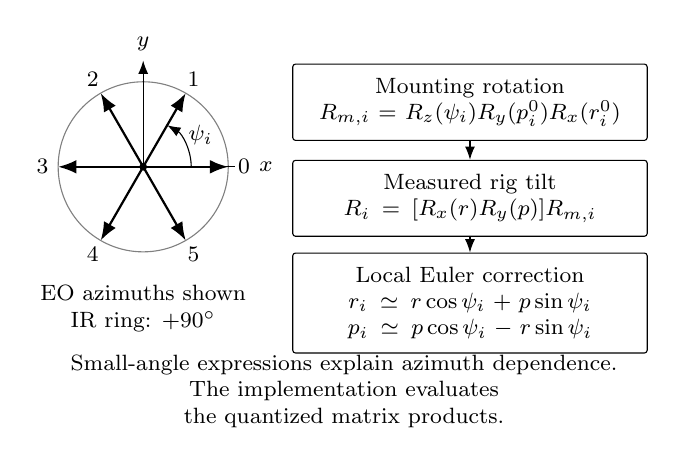
\begin{tikzpicture}[x=1cm,y=1cm,>=Latex,font=\footnotesize,
  glgbox/.style={draw,rounded corners=1pt,align=center,inner sep=5pt}]
  \draw[gray] (1.45,0) circle (1.08);
  \draw[->] (1.45,0)--(2.8,0) node[right] {$x$};
  \draw[->] (1.45,0)--(1.45,1.35) node[above] {$y$};
  \fill (1.45,0) circle (1.4pt);
  \foreach \a/\n in {0/0,60/1,120/2,180/3,240/4,300/5}{
    \draw[->,thick] (1.45,0)--++(\a:1.08);
    \node[fill=white,inner sep=1pt] at ($(1.45,0)+(\a:1.28)$) {\n};
  }
  \draw[->] (2.06,0) arc[start angle=0,end angle=60,radius=.61];
  \node at (2.18,.40) {$\psi_i$};
  \node[align=center] at (1.45,-1.80) {EO azimuths shown\\IR ring: $+90^\circ$};
  \node[glgbox,text width=4.15cm] (mount) at (5.60,.82)
    {Mounting rotation\\$R_{m,i}=R_z(\psi_i)R_y(p_i^0)R_x(r_i^0)$};
  \node[glgbox,text width=4.15cm] (body) at (5.60,-.40)
    {Measured rig tilt\\$R_i=[R_x(r)R_y(p)]R_{m,i}$};
  \draw[->] (mount)--(body);
  \node[glgbox,text width=4.15cm] (local) at (5.60,-1.73)
    {Local Euler correction\\$r_i\simeq r\cos\psi_i+p\sin\psi_i$\\
     $p_i\simeq p\cos\psi_i-r\sin\psi_i$};
  \draw[->] (body)--(local);
  \node[align=center,text width=7.8cm] at (4.0,-2.85)
    {Small-angle expressions explain azimuth dependence.\\
     The implementation evaluates the quantized matrix products.};
\end{tikzpicture}

\caption{Camera mounting orientation changes the local roll/pitch induced by
one rig tilt. The small-angle relation is explanatory; finite-angle values
come from the fixed-point matrix chain.}
\label{fig:gl_projection}
\end{figure}

The orientation trigonometric ROM contains $36000$ sine/cosine pairs at
$0.01^\circ$ spacing. Its scale is $32767$, including the matrix identity
entries. Each dot product uses the quantizer
\begin{equation}
 \begin{aligned}
 Q(a)&=\operatorname{sat}_{[-32768,32767]}
       \left(\left\lfloor\frac{a+2^{14}}{2^{15}}\right\rfloor\right),
 \\
 [AB]_{jk}&=Q\!\left(\sum_{\ell=0}^2 A_{j\ell}B_{\ell k}\right).
 \end{aligned}
 \label{eq:gl_mat_quant}
\end{equation}
The positive bias applies even to negative accumulators. Replacing it with
symmetric rounding, floating-point multiplication, or a reassociated matrix
chain changes the bit-level result. Products are signed 32-bit values and
the RTL accumulator is signed 36-bit. ROM generation uses the C library's
nearest rounding with half-way cases away from zero.

The inverse trigonometric operator $A(y,x)$ implements integer
$\operatorname{atan2}$ in centidegrees. For $m=\min(|x|,|y|)$ and
$d=\max(|x|,|y|)>0$, it indexes a $4097$-entry table by
\begin{equation}
 \begin{aligned}
 j&=\left\lfloor\frac{4096m+\lfloor d/2\rfloor}{d}\right\rfloor,\\
 L[j]&=\operatorname{round}_{\mathrm{away}}
       \left(\frac{18000}{\pi}\tan^{-1}\frac{j}{4096}\right).
 \end{aligned}
\end{equation}
Axis exchange and quadrant reconstruction give the complete angle;
$A(0,0)=0$. With $v=\operatorname{clip}(-R_{i,20},-32767,32767)$,
\begin{equation}
 p_i=A\!\left(v,\left\lfloor\sqrt{2^{30}-v^2}\right\rfloor\right).
\end{equation}
If the magnitude of the ROM cosine of $p_i$ exceeds $8$, then
$r_i=A(R_{i,21},R_{i,22})$ and
$y_i=A(R_{i,10},R_{i,00})$; otherwise $r_i=0$ and
$y_i=A(-R_{i,01},R_{i,11})$. The extracted yaw is not used by the renderer.
The $32767$ scale and integer square root mean that ideal right-angle
inputs need not yield exactly $9000$ cd.

\subsection{Correction Range and Preserved Pixel Mapping}
The controller first computes all six camera roll/pitch pairs and
$M=\max_i\{|r_i|,|p_i|\}$. When $(r,p)\ne(0,0)$ and $M>1000$, it replaces
each live component $v\in\{r,p\}$ by
\begin{equation}
 v'=\operatorname{sgn}(v)
   \left\lfloor\frac{1000|v|+\lfloor M/2\rfloor}{M}\right\rfloor
 \label{eq:gl_global_scale}
\end{equation}
and recomputes the six cameras once. Static trims are never rescaled.
This single global adjustment is distinct from independently clipping six
camera poses, and it need not force every recomputed angle within the limit.
A separate flag reports that condition. The preserved renderer finally
clips each camera roll and pitch to $[-1000,1000]$ cd. Disabled or unusable
live correction bypasses the projection and returns the static trim arrays
exactly; enabled zero tilt still executes the quantized matrix chain.

Let $\boldsymbol b(u,v)$ be the archived inverse map, in original source
pixels, with source center $(c_x,c_y)=(W/2,H/2)$. For the final camera
angles $\bar r_i,\bar p_i$ in degrees, the source coordinate is
\begin{align}
 t_i&=\operatorname{round}_{\mathrm{away}}(K_p\bar p_i/2^{16}),\\
 d_x&=b_x-c_x, & d_y&=b_y+t_i-c_y,\\
 x_s&=c\,d_x+s\,d_y+c_x,&
 y_s&=-s\,d_x+c\,d_y+c_y,
 \label{eq:gl_map_affine}
\end{align}
where $c=\cos(-\bar r_i)$, $s=\sin(-\bar r_i)$ and
$K_p=\operatorname{round}_{\mathrm{away}}(2^{16}k_p)$ is $-642253$ for EO
($k_p=-9.80$) or $-571474$ for IR ($k_p=-8.72$).
Translation precedes rotation.
This pixel path intentionally uses a different trigonometric scale,
$32768$, so zero angle is an exact identity. Its $1001$-entry magnitude
ROM covers $0$--$1000$ cd, restores signs at runtime, and stores the pitch
translation as a signed 8-bit integer ($\pm98$ EO or $\pm87$ IR rows).
The newer C optical path's resize-normalized EO factor is Q16
$-1140855$, approximately $-17.408$ pixels/degree; it is not substituted
into the retained renderer. Therefore exact agreement of the orientation
engine with C does not imply end-to-end pixel agreement with that newer
optical pipeline.

Map origins and running coordinates are signed 32-bit integers with
$16$ fractional bits. Each row segment has at most $64$ pixels; stored
16-bit increments have $5$ fractional bits for EO and $4$ for IR, and
are shifted left by $11$ or $12$ before transformation. Transformed
increments use signed 24-bit Q16 storage. Coordinate products are shifted
arithmetically by $15$ without an added rounding bias. Since the map is
affine within a segment, transformed endpoints bound every coordinate in it.

The sampler accepts $0\le x_s\le W-2$ and $0\le y_s\le H-2$; other
samples become black. It uses two vertically adjacent samples, rather than
general bilinear interpolation. EO quantizes the horizontal coordinate to
the output pixel's chroma parity and vertically interpolates luma and chroma
separately with a $2^{15}$ rounding bias before shifting by $16$. IR uses
$\lfloor x_s\rfloor$, truncating fixed-point vertical interpolation, and
constant chroma $128$. Archived seam-weight ROMs and strip placement remain
unchanged. EO overlaps contain $17$ output pixels; ordinary IR overlaps
contain $29$. The IR camera-2/3 fold seam uses the inherited $48$-pixel tail,
$90$-pixel head, and specialized alpha-index mapping.

\section{Frame-Coherent FPGA Architecture}
\label{sec:gl_architecture}
\label{sec:fpga}

\subsection{Atomic Pose Reception and Source-Epoch Association}
The runtime flow is shown in Fig.~\ref{fig:gl_runtime}.
The MCU writes I\textsuperscript{2}C slave address \texttt{0x36}, starting
at register \texttt{0x10}, with four little-endian bytes: signed 16-bit
roll followed by signed 16-bit pitch. The receiver commits only at STOP
after exactly four acknowledged sequential data bytes. Partial, excess,
misordered, or restarted bursts cannot publish a torn pose. A separate
one-byte transaction at \texttt{0x04} accepts \texttt{0xA1} to enable
correction and \texttt{0xA0} to disable it; reset is disabled. The MCU
enables correction only for UI On together with Attitude Sensor.
Request/acknowledge CDC mailboxes transfer coherent pose and control into
the DDR user-interface (UI) clock domain. The 32-bit receipt sequence counts
accepted FPGA pose transactions; it is not an IMU timestamp.

\begin{figure}[t]
\centering% Native vector artwork; requires tikz with arrows.meta and positioning.
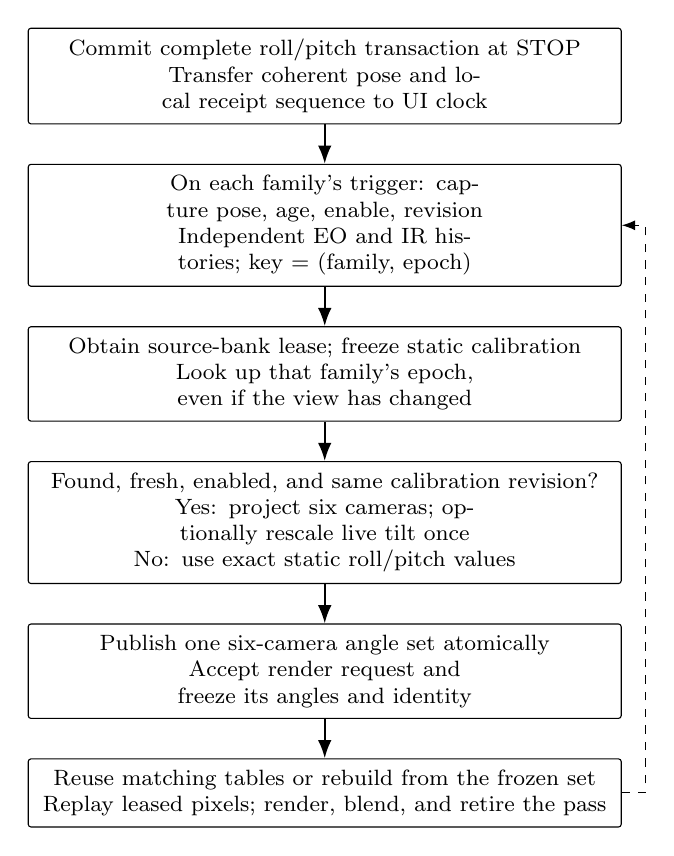
\begin{tikzpicture}[>=Latex,font=\footnotesize,node distance=5mm,
  glfbox/.style={draw,rounded corners=1pt,align=center,text width=7.25cm,inner sep=4pt},
  glflink/.style={->,thick}]
  \node[glfbox] (receive) {Commit complete roll/pitch transaction at STOP\\
    Transfer coherent pose and local receipt sequence to UI clock};
  \node[glfbox,below=of receive] (capture) {On each family's trigger: capture pose, age, enable, revision\\
    Independent EO and IR histories; key = (family, epoch)};
  \node[glfbox,below=of capture] (lease) {Obtain source-bank lease; freeze static calibration\\
    Look up that family's epoch, even if the view has changed};
  \node[glfbox,below=of lease] (policy) {Found, fresh, enabled, and same calibration revision?\\
    Yes: project six cameras; optionally rescale live tilt once\\
    No: use exact static roll/pitch values};
  \node[glfbox,below=of policy] (publish) {Publish one six-camera angle set atomically\\
    Accept render request and freeze its angles and identity};
  \node[glfbox,below=of publish] (render) {Reuse matching tables or rebuild from the frozen set\\
    Replay leased pixels; render, blend, and retire the pass};
  \foreach \a/\b in {receive/capture,capture/lease,lease/policy,policy/publish,publish/render}
    \draw[glflink] (\a)--(\b);
  \draw[->,dashed] (render.east)--++(.30,0)|-(capture.east);
\end{tikzpicture}

\caption{Pose selection follows the source-frame lease. New poses may arrive
throughout rendering but cannot modify an accepted pass. A lease or mode
change before acceptance cancels pending computation.}
\label{fig:gl_runtime}
\end{figure}

EO strobe and IR genlock drive independent 16-bit epoch counters. Each
family's six capture writers receive its Gray-coded epoch; a synchronized
trigger edge also captures the latest coherent pose in that family's
16-entry history. Each entry stores the complete epoch tag, roll/pitch,
receipt sequence, pose age, validity, enable state, and calibration revision.
Both histories continue capturing while the other family is displayed.
Consequently identical numeric EO and IR epochs cannot select each other's
pose. Full tags reject an entry overwritten by an index alias; requests
must not remain live across an entire 16-bit epoch wrap.

Pose age is zero on its receipt edge and increases in UI cycles. Freshness
is evaluated \emph{at trigger capture}, with the inclusive default bound
$23{,}340{,}000$ cycles ($100$ ms at nominal $233.4$ MHz).
Age is 32-bit saturating, with a sticky overflow flag that forces unusable
status. A pose update on the capture edge takes precedence; capture also
takes precedence over a simultaneous lookup of the same tag. Neither this
age bound nor an epoch establishes the physical exposure time. IMU filtering,
delivery latency, trigger-to-exposure delay, and their variation remain
separate calibration quantities.

The frameset manager provides source banks sharing an epoch among the
present cameras and holds the panorama lease until retirement. The pose
controller looks up the key (sensor family, leased epoch), freezes the
current static trims, and checks the captured calibration revision. Missing,
stale, disabled, or revision-mismatched data selects the exact static bypass.
The static register-bank path requires $2^{25}$ unchanged UI cycles before
adopting new values and clamps them to $\pm1000$ cd; the MCU accepts UI
trims within $\pm500$ cd. The two 16-bit bank-update counters form the
32-bit revision, so a change in either bank invalidates old calibration
association. This settling filter is distinct from the atomic live-pose
transaction protocol.

\subsection{Frozen Parameters and Source-Driven Rendering}
Figure~\ref{fig:gl_hardware} shows the implemented data and control paths.
One iterative projection engine evaluates six cameras sequentially and
publishes their $6\times16$-bit roll and pitch arrays atomically. At render
acceptance, the renderer snapshots those arrays, sensor selection, and
revision. Table construction reads the same frozen registers. Identical
angles and sensor selection permit table reuse; updates arriving during a
build or active pass cannot invalidate it. Replay is held until the new
source requirements are valid, avoiding a first-row fetch based on an old
table. The lease/pose controller cancels obsolete work before acceptance;
accepted coefficients remain fixed through completion or abort.

\begin{figure*}[t]
\centering% Native vector artwork; requires tikz with arrows.meta, positioning, calc.
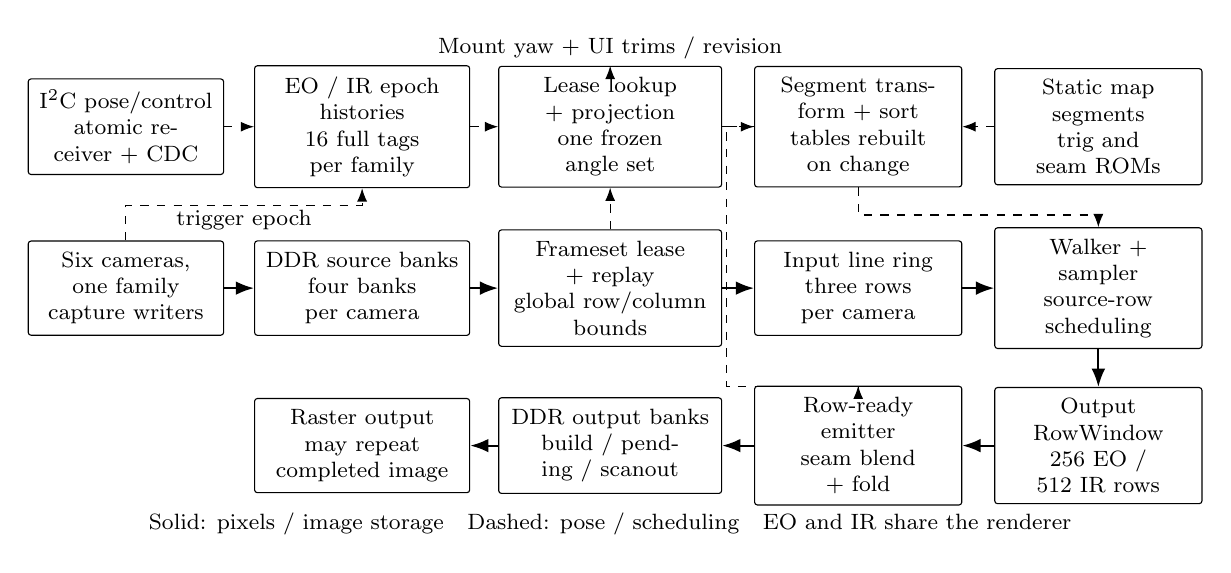
\begin{tikzpicture}[x=1cm,y=1cm,>=Latex,font=\footnotesize,
  glhbox/.style={draw,rounded corners=1pt,align=center,inner sep=4pt,minimum height=.90cm},
  glhdata/.style={->,thick},glhctrl/.style={->,dashed}]
  \node[glhbox,text width=2.20cm] (imu) at (1.25,0)
    {I$^2$C pose/control\\atomic receiver + CDC};
  \node[glhbox,text width=2.45cm] (hist) at (4.25,0)
    {EO / IR epoch histories\\16 full tags per family};
  \node[glhbox,text width=2.55cm] (pose) at (7.40,0)
    {Lease lookup + projection\\one frozen angle set};
  \node[glhbox,text width=2.35cm] (table) at (10.55,0)
    {Segment transform + sort\\tables rebuilt on change};
  \node[glhbox,text width=2.35cm] (rom) at (13.60,0)
    {Static map segments\\trig and seam ROMs};
  \draw[glhctrl] (imu)--(hist);
  \draw[glhctrl] (hist)--(pose);
  \draw[glhctrl] (pose)--(table);
  \draw[glhctrl] (rom)--(table);
  \node[align=center] (cal) at (7.40,1.0) {Mount yaw + UI trims / revision};
  \draw[glhctrl] (cal)--(pose);
  \node[glhbox,text width=2.20cm] (camera) at (1.25,-2.05)
    {Six cameras, one family\\capture writers};
  \node[glhbox,text width=2.45cm] (ddr) at (4.25,-2.05)
    {DDR source banks\\four banks per camera};
  \node[glhbox,text width=2.55cm] (replay) at (7.40,-2.05)
    {Frameset lease + replay\\global row/column bounds};
  \node[glhbox,text width=2.35cm] (ring) at (10.55,-2.05)
    {Input line ring\\three rows per camera};
  \node[glhbox,text width=2.35cm] (walk) at (13.60,-2.05)
    {Walker + sampler\\source-row scheduling};
  \foreach \a/\b in {camera/ddr,ddr/replay,replay/ring,ring/walk}
    \draw[glhdata] (\a)--(\b);
  \draw[glhctrl] (camera.north)--++(0,.45)-|(hist.south);
  \node[fill=white,inner sep=1pt] at (2.75,-1.19) {trigger epoch};
  \draw[glhctrl] (replay)--(pose);
  \draw[glhctrl] (table.south)--++(0,-.35)-|(walk.north);
  \node[glhbox,text width=2.35cm] (window) at (13.60,-4.05)
    {Output RowWindow\\256 EO / 512 IR rows};
  \node[glhbox,text width=2.35cm] (emit) at (10.55,-4.05)
    {Row-ready emitter\\seam blend + fold};
  \node[glhbox,text width=2.55cm] (out) at (7.40,-4.05)
    {DDR output banks\\build / pending / scanout};
  \node[glhbox,text width=2.45cm] (scan) at (4.25,-4.05)
    {Raster output\\may repeat completed image};
  \foreach \a/\b in {walk/window,window/emit,emit/out,out/scan}
    \draw[glhdata] (\a)--(\b);
  \draw[glhctrl] (table.west)--++(-.35,0)--++(0,-3.30)-|(emit.north);
  \node[align=center] at (7.40,-5.05)
    {Solid: pixels / image storage\quad Dashed: pose / scheduling\quad EO and IR share the renderer};
\end{tikzpicture}

\caption{Implemented panorama path. Full source-frame address spaces reside
in DDR even when EO capture writes a proven subwindow. On-chip input rows
are replay caches, not the complete image storage. The same processing
engine serves EO or IR; output scanout is decoupled from image production.}
\label{fig:gl_hardware}
\end{figure*}

The base map contains $480\times6\times11=31680$ EO segments or
$480\times6\times10=28800$ IR segments. The table builder transforms each
segment, chooses traversal direction so source $y$ is nondecreasing, and
counting-sorts entries by their first source row. It stores a bucket end
index for each source row and a row-ready threshold equal to the maximum
last source row needed by each output row. A $4096$-entry queue retains
partially traversed segments. For source row $y_0$, the walker drains the
previously queued work and newly eligible segments, emits their pixels,
and requeues unfinished segments. Coordinates advance by addition.

DDR replay fills a three-row ring for each camera: rows $y_0$ and $y_0+1$
are sampled while $y_0+2$ is prefetched into the third slot. After pipeline
drain, the retired row's slot may be reused. The physical ring contains
$18$ memories of $512\times64$ bits, of which $480$ words cover an EO row.
Partially completed output strips are stored in a $2^{18}\times72$-bit
UltraRAM RowWindow. Packing four 16-bit EO pixels per word gives $256$
output-row slots; packing eight 8-bit IR samples gives $512$. The parameter
store is $32768\times144$ bits and the work queue $4096\times144$ bits.
These structures, ROMs, and metadata must all be included in memory claims;
the design is not a strict two-line architecture.

An output row becomes eligible only after all its required source rows
have retired. The emitter then blends seams and folds the panorama into
two HD raster bands. EO divides $3840$ columns into two $1920$-pixel halves.
IR divides its $3576$ valid columns into two $1788$-pixel halves and pads
each to $1920$ pixels. Both use $960$ active output rows within a
$1920\times1080$ raster. RowWindow alias guards stall the walker when the
emitter can advance; an unresolvable window overflow is reported and the
affected output row is blackened. It is not silently treated as a valid
stabilized image.

\subsection{Capture Coverage, Bandwidth, and Validation Boundary}
Each camera has four DDR source-bank address spaces. EO panorama capture
uses rows $0$--$1079$ and 16-pixel beats $8$--$111$, namely columns
$128$--$1791$. This fixed envelope includes every permitted transformed
segment endpoint, the sampler guard, and replay's eight-beat rounding for
all $2001$ roll values and pitch translations between $-98$ and $98$ rows.
Pitch monotonicity at fixed roll and affine variation within a segment
reduce the proof to endpoint tests at the two pitch extremes. IR retains
full $640\times512$ capture. A selected EO single-camera view requests full
capture and waits for a descriptor marked as adopting the full window;
an old narrow descriptor cannot satisfy it. The marker denotes the adopted
window, not an independent proof of a complete received raster.

Capture and output writes share DDR service. At an \emph{assumed} $30$
new frames/s, EO panorama capture requires $20.2176$ million useful
256-bit write beats/s, and output construction adds $3.456$, totaling
$23.6736$. IR panorama totals $1.8432+3.456=5.2992$ million beats/s.
The families' DDR captures are mutually gated in steady state. A historical
aggregate write measurement of $22.3$ million beats/s is below the EO
requirement and is not a measurement of this candidate. These write totals
exclude read service and do not establish sustainable frame rate. Output
scanout may repeat a completed image, so raster rate must be distinguished
from unique-content rate. A per-row capture ROM alone would not remove
this burden while replay requests its present global rectangular bounds.

Verification of the arithmetic, frame association, and renderer is reported in
Section~\ref{sec:verification}; measured and routed results follow in
Section~\ref{sec:hardware}.

\section{Numerical and Temporal Verification}
\label{sec:verification}
\subsection{Separate Oracles for Angles and Pixels}
The ten-suite regression was rerun on October 23, 2026 at source revision
\code{5126c37}. Full hashes, commands, inputs, and logs are archived with the
paper. Results below refer to this run unless a historical scope is stated.

The orientation reference is extracted from the compiled C++ translation
unit, with source and table hashes recorded. A portable C++ harness is
compiled using MSVC with precise floating-point semantics for table
construction; an independently expressed Python model checks the integer
operations. The 79,397 requests compare 245,237 integer outputs, including
inverse-trigonometric boundaries, division, integer square root, signed
extremes, directed camera cases, and 2,000 seeded random frames. All recorded
outputs agree exactly. This establishes agreement with the chosen discrete
reference, not agreement with ideal real-valued rotations or measured rig
orientation.

The pixel oracle is separate. It uses the preserved EO/IR segment maps and
sampling arithmetic, rather than the newer C application's optical profile.
Two renderer suites exercise legacy static input and the frozen gravity-pose
interface. Each compares 14,112,000 pixels exactly across EO and IR cases,
including zero, mixed, and limit-angle configurations. Consequently angle
agreement and pixel agreement are not conflated into an unsupported claim
of end-to-end equality to a different optical pipeline.

\begin{table}[t]
\centering\footnotesize
\caption{Recorded verification scopes and outcomes. Counts refer to tested
cases, not exhaustive coverage of the complete system state space.}
\label{tab:verification}
\begin{tabularx}{\columnwidth}{@{}lY@{}}
\toprule
Scope & Check and observed result \\
\midrule
C/Python arithmetic & 79,397 requests; 245,237 integer outputs agree \\
Camera projection RTL & 1,342 compiled-C vectors; exact outputs \\
Six-camera controller & 266 cases; atomic publication and limiting \\
Pose association & 21 lease cases; independent EO/IR histories, cancellation, fallback \\
Trigger epoch & Phase/reset tests; all 65,536 counter increments \\
I\textsuperscript{2}C interface & 109 wire-level checks; partial/malformed transaction rejection \\
CDC mailbox & Three clock ratios, clock stoppage, reset and coherent transfer \\
Renderer & Two suites, each 14,112,000 matching pixels; eight table cases \\
Capture/selection & 116 envelope checks; 19 single-selection checks; marker-order test \\
\bottomrule
\end{tabularx}
\end{table}

\subsection{State Invariants and Failure Cases}
Table~\ref{tab:verification} complements numeric tests with transaction and
state-machine tests. Publication occurs only after a complete pose burst;
changing input registers while computation is busy cannot change its result.
A source lease selects the corresponding family's history entry, not the
newest pose and not an equal numeric epoch from the other sensor family.
Missing, stale, disabled, overwritten, and calibration-mismatched entries
exercise the static fallback. Mode and lease changes cancel pending work,
while reset clears valid state. The renderer tests vary live inputs during
table generation and replay to check that accepted coefficients remain
constant.

The capture-envelope check has a different character: affine coordinates
within each segment and pitch monotonicity reduce a bounded geometric
coverage problem to endpoint checks over the supported discrete roll range.
This proves coverage of the defined fetch envelope under those model
assumptions. It does not prove that camera capture, DDR arbitration, source
bank ownership, and display publication meet every real-time deadline.
Likewise functional CDC tests do not prove metastability margins; those
require implementation constraints and physical review.

The orientation engine takes 531--601 clock cycles in the camera tests; the
enabled six-camera controller takes 3,556--7,319 cycles, depending on whether
the global rescale needs a second pass. At the nominal 233.4 MHz UI clock,
that controller range corresponds to approximately 15.2--31.4 microseconds.
This is a conversion of simulation cycles, not a measured camera-to-display
latency, and excludes table building, source replay, memory contention,
publication, and scanout. The firmware control and calibration-storage tests
are archived separately; they do not validate the physical filter response.

\section{Archived Static Stitching Evaluation}
\label{sec:legacy-evaluation}
We evaluate saved software outputs from the calibrated panorama pipeline
and three image-based baselines. This is an analysis of existing outputs, not a new run of
the renderers or neural networks. Its scope is pre-blend photometric consistency
between warped views of this calibrated rig; it does not measure temporal
stabilization, absolute gravity alignment, or the integrated FPGA output.

\subsection{Cases, Configurations, and Metrics}
The archive contains six named EO cases with six source views. The StabStitch++ wrapper evaluates cameras 0--2. We therefore use a
shared target set of 12 case/pair identities for all four methods: pairs
$(0,1)$ and $(1,2)$ in each case. The wraparound pair $(5,0)$ is outside this evaluation. The six case names
identify configurations; they do not establish six statistically independent
scenes or acquisitions.

The saved UDIS++ configuration requests 30 iterations of per-pair adaptation,
and the associated code contains optimizer updates \cite{nie2023parallax}.
StabStitch++ is supplied with 16 repetitions of each static input image to
satisfy the temporal interface \cite{nie2025stabstitch2}. Its results here
therefore test static alignment under that wrapper, not its video-stability
capability. The preparation script undistorts the image-based inputs using
the recorded intrinsics. The calibrated renderer additionally uses mounting
geometry and inertial angles, so the methods still receive different priors.

We preserve the archived metric formula. Images are converted to grayscale;
the overlap mask is eroded by a $5\times5$ square. PSNR and the mean local SSIM
map \cite{wang2004ssim} are evaluated over that mask, both directly and after
Gaussian smoothing with $\sigma=2$ output pixels. We call the latter
\emph{smoothed} scores, not independent measures of geometric error. Each
reported mean weights case/pair identities equally. The calibrated renderer,
UDIS++, and StabStitch++ scores are recomputed from saved warped images; SIFT
scores are retained from the saved evaluator JSON, which used its original
in-memory masks.

This protocol has material limitations. The calibrated renderer infers validity
from image intensity, whereas the baselines use saved masks. Output scales,
canvases, compression, and visible regions differ, so Gaussian smoothing with
$\sigma=2$ pixels does not represent a shared angular scale. Exposure, texture, parallax,
and smoothing affect both metrics. Consequently these scores describe the saved
outputs under their original evaluation conventions; they are neither
ground-truth registration errors nor a controlled ranking of the methods.

\begin{table}[t]
\centering
\caption{All 12 shared target identities. Scores are means over each method's
successful outputs; raw/smoothed values are separated by a slash. The SIFT row
has a different successful subset and is not directly comparable as a paired
mean. Different masks and scales remain throughout.}
\label{tab:legacy-targets}
\small
\setlength{\tabcolsep}{3pt}
\begin{tabular}{lccc}
\toprule
Method & Valid/target & PSNR (dB) & SSIM \\
\midrule
Calibrated G-locked & 12/12 & 15.05/22.59 & .311/.752 \\
UDIS++ & 12/12 & 13.47/16.88 & .205/.424 \\
StabStitch++ & 12/12 & 12.82/15.56 & .213/.450 \\
SIFT + homography & 9/12 & 13.24/16.16 & .304/.534 \\
\bottomrule
\end{tabular}
\end{table}

\subsection{Matched Identities and Retained Failures}
Table~\ref{tab:legacy-targets} reports coverage before any common-success
selection. The SIFT evaluator records failures for case
\texttt{EO\_Test2\_R\_2.15\_P\_0}, pair $(0,1)$;
\texttt{EO\_Test5\_R\_4.75\_P\_-4.5}, pair $(1,2)$; and
\texttt{EO\_Test6\_R\_1.25\_P\_6.5}, pair $(0,1)$.
We retain these failures explicitly instead of assigning an arbitrary metric
value or treating absent scores as successful measurements.

Figure~\ref{fig:legacy-matched} restricts all four methods to the nine identical
case/pair identities with available successful scores. Smoothed PSNR/SSIM are
$22.56$/.757 for G-locked, $17.09$/.442 for UDIS++, $15.60$/.466 for
StabStitch++, and $16.16$/.534 for SIFT. G-locked has higher recorded values on
this conditional subset. Matching identities controls the sampled camera pairs, but not the mask,
scale, or information differences described
above. These descriptive means do not support statistical significance or
generalization claims. No IR baseline runs were found in this comparison
archive, so it cannot establish comparative IR generalization.

\begin{figure}[t]
\centering
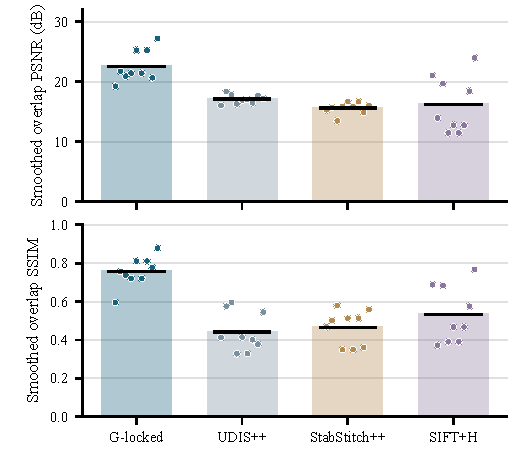
\includegraphics[width=\columnwidth]{figures/legacy_matched_comparison.pdf}
\caption{Saved-output comparison on nine common-success case/pair identities;
dots represent individual pairs and horizontal lines their means.
Coverage is reported against the 12-target set. Masks, output scales, and
calibration access differ across methods. These conditional photometric scores
do not measure temporal stabilization or independent geometric accuracy.}
\label{fig:legacy-matched}
\end{figure}

The accompanying reanalysis script, per-seam CSV, and JSON manifest record
target identities, failures, software versions, source-file hashes, and the
metric conventions. They reproduce the summary when the identified local
archive is supplied; the raw captures and original model runs are not included
in this paper repository. The next evaluation step is to use independently
measured geometry and synchronized dynamic captures, with common output scale,
validity support, and a declared adaptation budget.

\section{Archived Video Evaluation}
\label{sec:video-evaluation}
\subsection{Saved Outputs and Comparator}
We re-evaluate three saved indoor panorama videos: uncorrected output,
camera-specific inertial correction, and a rigid optical-flow comparator.
Each contains 1800 encoded frames at $1900\times540$ pixels and 30~frames/s,
covering three camera views. These software outputs do not exercise the
current FPGA. Correspondence by encoded frame index does not establish
exposure alignment or an independently acquired image at every index.

The available inertial generator performs undistortion and cylindrical
remapping, quantizes rig roll/pitch to $0.25^\circ$, projects those angles to
each camera, applies pitch and then roll warps, and concatenates cropped
strips without seam blending. Its pitch factor is $-19.6$ full-resolution
pixels/degree; the default output scale is one half. These operations differ
from the fixed-point mapper and blend pipeline in Section~\ref{sec:algorithm}.
No generation-command manifest identifies the selected three-view videos;
available logs describe four-view outputs. Reproducibility therefore concerns
measurement of the hashed saved videos, rather than their exact regeneration.

The flow implementation tracks Shi--Tomasi features with Lucas--Kanade flow,
fits a partial affine transform, and discards fitted scale. It smooths the
accumulated trajectory with a centered 61-tap Gaussian ($\sigma=15$ frames),
then applies rigid warps in a second pass. This offline comparator smooths a
relative path rather than referencing gravity; it is neither causal nor
representative of all spatially varying stabilizers.

\subsection{Paired Physical-Marker Measurements}
We detect an ArUco marker with the archived \code{DICT\_6X6\_250} procedure
using OpenCV 4.8.0 default detector parameters, including no corner refinement.
For each successful detection, the estimator averages the top- and bottom-edge
image angles and folds the result into $[-45^\circ,45^\circ)$. Every detected
marker in the evaluated windows is ID~15, with no multiple-marker detections.
For each interval we retain only indices at which all three methods detect
that ID. If $\mathcal I$ is this common set and $\theta_{m,i}$ is the edge-angle
estimate for method $m$, we report
\begin{equation}
 \sigma_{\theta,m}=\sqrt{\frac{1}{|\mathcal I|}
 \sum_{i\in\mathcal I}(\theta_{m,i}-\bar\theta_m)^2},
 \qquad
 \bar\theta_m=\frac{1}{|\mathcal I|}\sum_{i\in\mathcal I}\theta_{m,i}.
 \label{eq:markerstd}
\end{equation}
This population standard deviation measures image-orientation steadiness.
It does not measure bias relative to gravity or calibrated marker pose.
Perspective, remapping, compression, and integer corner localization contribute
to the measured variation.

\begin{table}[t]
\centering
\caption{Marker image-angle standard deviation on identical encoded indices
and marker ID~15. Each interval requests 450 frames. Values are descriptive
within these selected, temporally correlated sequences.}
\label{tab:marker-paired}
\small
\setlength{\tabcolsep}{4pt}
\begin{tabular}{lcccc}
\toprule
Interval & Common & Raw & IMU & Rigid flow \\
(s) & frames & ($^\circ$) & ($^\circ$) & ($^\circ$) \\
\midrule
5--20 & 444/450 & 6.092 & 1.317 & 5.830 \\
30--45 & 448/450 & 7.410 & 1.177 & 7.079 \\
\bottomrule
\end{tabular}
\end{table}

Raw, IMU, and flow yield 449/449/450 detections for 30--45~s and 445/450/449
for 5--20~s. Different missing indices leave 448 and 444 common frames.
Table~\ref{tab:marker-paired} and Fig.~\ref{fig:marker-traces} show lower
orientation variation for the saved IMU output in both intervals.
The means for 30--45~s are
$-3.777^\circ$, $-3.912^\circ$, and $-3.768^\circ$ for raw, IMU, and flow;
subtracting them for the plot does not establish a zero-gravity reference.
The archive includes interval-selection code based on motion and image/IMU
correlation. These selected, correlated frames are not independent held-out
trials; no significance or generalization claim is made.

\begin{figure}[t]
\centering
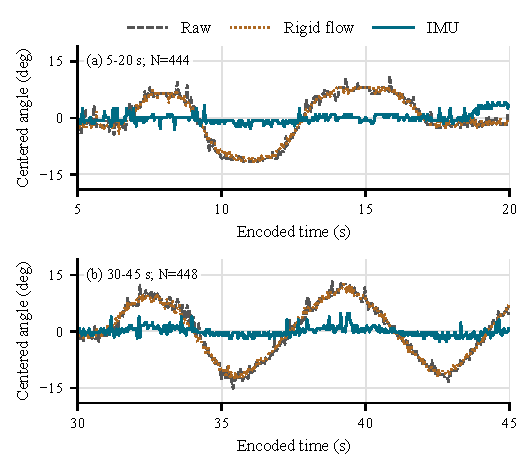
\includegraphics[width=\columnwidth]{figures/archived_marker_steadiness.pdf}
\caption{Physical-marker image orientation in two archived indoor intervals.
Each trace has its own common-support mean removed; gaps retain excluded
indices. The smaller variation of the IMU output is a saved-software result,
not a measurement of current FPGA leveling accuracy or absolute gravity.}
\label{fig:marker-traces}
\end{figure}

\subsection{Scope of the Inertial Diagnostics}
The archive also contains painted horizon and offline IMU-filter diagnostics.
A line derived from accelerometer attitude and the same
camera geometry used for correction tests model consistency, not an
independent physical horizon. The red-pixel extractor also selects scene
objects, demonstrably contaminating an indoor frame. The audit retains these
pixel statistics and support, without converting them through a nominal
pixels/degree constant into physical leveling errors.

The archived acquisition logs identify a RealSense D435i IMU, whereas the
current MCU uses the IIM46234 configuration in Section~\ref{sec:algorithm}.
The old filter comparison uses accelerometer angles from the same sensor as
its reference, includes centered five-sample averaging, and converts
correlation index shifts through a median sample interval despite irregular
timestamps. It cannot establish independent attitude accuracy, causal filter
delay, or the current system's latency. These diagnostics are retained for
reproduction, while hardware timing claims use the identified event boundaries
in Section~\ref{sec:hardware}.

\section{Hardware Implementation and Measurement}
\label{sec:hardware}

\subsection{Evidence and Implementation Configuration}
We separate four forms of evidence: fixed-point and protocol regression, placed-and-routed implementation, archived live pipeline measurements, and camera-input measurements. The authors additionally report successful qualitative operation of the integrated gravity path. Because that report is not accompanied by an identified image and a numerical motion trace, it does not supply a dynamic leveling-error, throughput, or latency statistic. Historical observations below retain their original build and measurement boundary. The accompanying evidence manifest records source paths, SHA-256 hashes, decoded timing words, and workbook checks.

A fresh full synthesis, placement, and routing run of source revision \code{5126c37} completed on October 23, 2026 using Vivado 2025.2 for an XCKU15P-FFVE1517-2-I. Table~\ref{tab:hw_resources} gives the complete top-level allocation, including DDR infrastructure, video interfaces, maps, and debug logic. These counts are not an incremental gravity-transform cost. The 58,523 register resources comprise 58,522 flip-flops and one register used as an AND/OR; no latches are reported. The 495 BRAM tiles comprise 492 RAMB36 and six RAMB18 primitives.

\begin{table}[t]
\centering
\caption{Whole-design routed resources, October 23 fresh gravity build.}
\label{tab:hw_resources}
\small
\begin{tabular}{lrrr}
\toprule
Resource & Used & Available & Utilization \\
\midrule
CLB LUTs & 54,321 & 522,720 & 10.39\% \\
CLB registers & 58,523 & 1,045,440 & 5.60\% \\
BRAM tiles & 495 & 984 & 50.30\% \\
URAM blocks & 92 & 128 & 71.88\% \\
DSP48E2 & 30 & 1,968 & 1.52\% \\
\bottomrule
\end{tabular}
\end{table}

The UI clock is 233.380 MHz, the HD video clock is 74.250 MHz, and the reference is 27 MHz. Routed setup, hold, and pulse-width worst slacks are respectively $+0.022$, $+0.010$, and $+0.009$ ns, with zero total negative slack in each summary. All 143,180 routable nets are fully routed, and no Error-severity DRC entry is reported. The scoped gravity and IR-epoch audit covers 3,524 sequential cells without missing clocks, unconstrained internal paths, or unintended internal timing cuts. The 64-bit pose and eight-bit control mailbox transfers retain their 4.000 ns maximum-delay constraints; all 80 reported bus-skew checks pass, with a minimum slack of $+2.525$ ns.

These checks establish closure under the reported internal constraints, not complete physical signoff. The full-design CDC report retains 131 Critical and 265 Warning entries, including inherited crossings requiring separate disposition. The timing report also identifies 159 inputs without input-delay constraints and 37 output-delay check entries (36 unconstrained outputs plus one clock port). Consequently, neither the scoped mailbox checks nor positive internal slack proves board-I/O timing or exposure synchronization. C/RTL regressions complement these implementation checks by testing angle arithmetic, coherent pose transport, epoch association, and rendered pixels; simulation does not measure external-memory stalls or camera timing.

\subsection{Storage and Throughput Boundaries}
The implemented pipeline stores captured source frames and published output frames in DDR. Replay feeds a three-row source ring, followed by the source-driven sampler and a 256-row EO (512-row IR) destination RowWindow. Vertical interpolation accesses two adjacent source rows, but the complete architecture is not a two-line-only streaming pipeline. Memory accounting must include primitive rounding, control, metadata, external frame storage, and debug. The nominal capacity represented by the routed BRAM and URAM allocation is 5,672,448 bytes including parity; that number includes infrastructure and excludes DDR and distributed memory, so it is not directly comparable with an algorithm's image or model-memory footprint.

Table~\ref{tab:historical_fps} reports the accepted September 4, 2026 static-renderer run, build \code{c83e29d}. Distinct images were counted by exact image hashes in nominal 60 FPS HD-SDI/USB captures; EO output was also checked against a \code{frame\_done} counter. These measurements distinguish output updates from repeated scanout rasters. They demonstrate near-30 updates/s for the recorded configuration, with no black grabs in these finite samples.

\begin{table}[t]
\centering
\caption{Archived static-renderer output measurements; these are not current gravity-envelope benchmarks.}
\label{tab:historical_fps}
\small
\begin{tabular}{lrr}
\toprule
Mode & Distinct images/s & Black grabs / total \\
\midrule
EO panorama & 29.97 & 0 / 598 \\
IR panorama & 29.70 & 0 / 474 \\
EO single & 29.95 & 0 / 477 \\
IR single & 29.95 & 0 / 477 \\
\bottomrule
\end{tabular}
\end{table}

The historical EO capture window was 88 beats by 1,008 rows; the gravity envelope is 104 beats by 1,080 rows. At 30 updates/s, six-camera capture requires 20.218 million write beats/s, while output publication adds 3.456 million, for 23.674 million aggregate write beats/s. Each beat carries 32 useful pixel bytes, giving 757.555 MB/s of analytical write demand before reads and protocol overhead. The older run observed approximately 22.3 million aggregate write beats/s, including capture and output. That observation is neither a capture-only budget nor a proven bandwidth ceiling. The wider envelope's sustained rate must be measured independently. Although the DDR UI is 384 bits wide, the pixel path uses 256 payload bits per beat; clock rate multiplied by the physical interface width would overstate useful pixel throughput. Likewise, the archived reduction from 29.8 to 17.9 ms after reducing the fetch window describes render-pass service time, not end-to-end video latency.

\subsection{Archived Event-Timing Measurements}
The August 19, 2026 captures use the V19 timing probe from revision \code{67955bc}. Its nominal timer tick is $64/233.4\,\mathrm{MHz}=0.274207\,\mu\mathrm{s}$. The event timestamp available at copy start is retained, and the interval ends at output-frame commit. Commit publishes a completed output buffer; it is not a display-scanout event. Table~\ref{tab:latency_snapshots} decodes the exact archived register words using that revision's field definitions.

\begin{table}[t]
\centering
\caption{Trace-backed last-event timing snapshots, revision \code{67955bc}. Values are event-to-output-commit intervals, not end-to-end latency.}
\label{tab:latency_snapshots}
\small
\begin{tabularx}{\columnwidth}{lYr}
\toprule
Mode & Start event & Interval (ms) \\
\midrule
EO single & Selected camera descriptor-valid & 16.294 \\
EO panorama & Newest camera-0 descriptor-valid & 63.505 \\
IR single & Selected camera frame pulse & 58.916 \\
\bottomrule
\end{tabularx}
\end{table}

Both EO captures hold a single timing word across all 2,048 ILA samples. The IR capture holds two values separated by one timer tick, both rounding to 58.916 ms. Repeated observations of a held last-event register are not independent frame-latency samples; these traces therefore do not support a latency distribution or a 95th percentile. The companion IR panorama file contains no sampled timing data and is omitted.

The boundaries also differ by mode. EO starts from a descriptor-valid event, whereas IR starts from a camera frame pulse. More importantly, the EO panorama timestamp is the newest camera-0 completion, not an identity-matched timestamp of the leased frameset. If that completion is newer than the leased content, the reported interval understates the selected source's age. It must not be interpreted as a validated capture-to-output delay for that source. The probe's copy-done field has a coarser 1.123153 ms bin width, and does not justify sub-0.1 ms copy-time precision.

The contemporaneous narrative lists other session observations and estimates a ``typical'' total by adding 16.7 ms mean row age and 16.7 ms scanout. Those additions are modeled terms, omit sensor/ISP delay, and do not remedy the panorama source association. We retain only the trace-backed snapshots as measured values. None of these historical intervals is a measurement of current gravity-path latency or physical exposure-to-display delay.

\subsection{Camera Raster and Content Synchronization}
Camera-input evidence is separate from renderer output FPS. The October 9 study used physical cameras 2--6 at 1080p60, manual shutter setting 1/60 s, gain 0 dB, zero external-trigger delay, and a 30 Hz FPGA trigger with 2 ms high time. The archived receiver detects a raster boundary at the first valid embedded BT.1120 timing marker whose V bit changes from one to zero, using the qualified rising-edge sampling path. A common nominal 27 MHz counter timestamps the resulting event after synchronization and before serialization. This observes a received-raster boundary, not a sensor exposure or an external VSYNC-pin edge. The shutter value is a verified setting, not a measured exposure duration, and the trigger timestamp observes the FPGA output rather than camera acceptance.

For each matched raster set, let $t_i$ be a camera timestamp and $P$ the estimated raster period. We sort $t_i\bmod P$ and subtract the largest circular inter-camera gap from $P$. This yields the shortest circular arc containing the five raster phases. Table~\ref{tab:camera_sync} summarizes the resulting spread for sequential 2D+3D digital noise reduction (DNR) settings. The audit independently recomputed all 14,051 spans from stored timestamps and periods, then reconciled the twenty corresponding workbook summary cells without modifying the workbook.

\begin{table}[t]
\centering
\caption{Five-camera raster-phase spread, October 9, 2026. DNR conditions were sequential; percentiles describe raster cohorts, not latency.}
\label{tab:camera_sync}
\small
\begin{tabular}{lrrrr}
\toprule
DNR condition & Sets & Median & p95 & Maximum \\
 & & \multicolumn{3}{c}{Spread (ms)} \\
\midrule
ON initial & 3,515 & 10.855 & 10.874 & 10.876 \\
OFF & 3,523 & 10.670 & 10.690 & 10.692 \\
ON return & 3,478 & 10.478 & 10.505 & 10.507 \\
OFF repeat & 3,535 & 10.252 & 10.272 & 10.274 \\
\bottomrule
\end{tabular}
\end{table}

Each condition spans approximately 58--59 s. Spread decreases through the return to DNR ON, so this sequence does not isolate a causal benefit from turning DNR OFF. Camera-clock drift remains a confounder. Small residuals after fitting that drift are not the actual five-camera spread. Moreover, matching periodic raster events cannot identify an unknown whole-frame pipeline offset. The approximately 10 ms spread therefore describes received raster phases, not aligned exposures.

Frozen-scene controls are essential to interpreting content signatures. Earlier full-frame signature measurements that suggested 60 fresh images/s continued changing under Freeze and were withdrawn. Later matched full-frame/ROI controls qualify cameras 2--4, whose live content changes occur predominantly every two input rasters, approximately 30/s despite approximately 60 rasters/s. Cameras 5 and 6 still show full-frame changes when frozen: 981 and 1,268 transitions with DNR ON, and 625 and 1,847 with DNR OFF, while frozen ROI signatures remain stable. Extra live ROI transitions also remain. Thus a full-frame change count cannot certify 60 independent clean images/s across the camera set, and disabling DNR does not resolve the diagnostic limitation.

Together, these records establish configuration-specific output update rates, input raster/content behavior, and event timing. They do not establish absolute exposure alignment. A quantitative dynamic gravity experiment must additionally identify the FPGA/MCU images, associate source and output identities, capture an independent orientation reference, and measure the desired exposure-to-output or exposure-to-display boundary under sustained load.

\section{Discussion and Qualification Limits}
\label{sec:discussion}
\subsection{What the Evidence Establishes}
The numerical tests support the specified discrete transformation, including cases where an intuitive floating-point replacement would differ by signed rounding or limiting order. Renderer pixel comparisons establish consistency with the preserved optical model. Source/pose tests show that accepted pass state is frozen and that invalid associations fall back to static correction. Routing establishes that the constrained implementation meets the reported timing checks on the selected device. These are complementary results, with distinct oracles and scopes.

The saved software outputs provide static alignment comparisons and paired physical-marker orientation measurements. The latter show lower image-angle variation for the saved inertial output in two selected intervals, without an independent gravity reference. These experiments do not test the current FPGA pixel path, which intentionally retains older optical maps, or the current live inertial loop. Likewise, historical FPS and latency measurements demonstrate behavior of their recorded builds. Their utility for this design is to identify repeated-camera frames, buffer publication delay, and bandwidth pressure that a purely geometric validation would miss.

\subsection{Limits of the Motion and Sensor Model}
Only rig roll and pitch enter the live rotation. Yaw heading stabilization, depth-dependent translation, rolling-shutter compensation, and inter-camera radiometric correction are outside this model. The affine source-map correction is an approximation whose acceptable error depends on field of view, tilt, crop, and scene depth. Saturation retains memory safety but can leave residual geometric error. A one-pass global limiter is not a proof that every camera output lies within the renderer envelope when mounting trims are nonzero.

The selected mounting profile and the preserved optical maps have separate provenance. Changing optical focal parameters, pitch scale, or crop requires regenerating and verifying the maps, signed shift widths, and capture envelope together. Dynamic UI roll/pitch trims are supported; saving a yaw value does not change the current RTL's fixed mounting yaw. A stored calibration marker prevents first-start defaults from overwriting subsequent UI edits, but a programmer mass erase removes that state.

\subsection{Dynamic Validation Still Required}
The authors' qualitative report of live functionality is consistent with the implementation intent, but does not supply an error distribution or a reproducible image/firmware identity. A quantitative test should record the FPGA bitstream/probe hashes, MCU image, actual trim banks, camera format, exposure, trigger delay, DNR state, and measured source and output rates. A fixed rig motion profile and an independent orientation reference should be captured together with source-exposure and displayed-frame identities. Report both leveling and temporal smoothness because suppressing low-frequency gravity error and smoothing relative image motion are different objectives.

At minimum, compare stabilization Off/On on identical motions; test receipt-time versus frame-associated pose; exercise the static fallback and calibration update boundaries; and repeat under DDR stalls and each sensor family. Measure angle error, valid area, seam disagreement, distinct-frame throughput, and event-to-event latency with distributions across repeated runs. Controlled exposure timing is necessary when comparing camera synchronization: raster-start alignment alone can remain good while exposure or ISP latency changes. A current-build sensor-to-display latency claim requires the complete acquisition/processing/scanout path to be observed, rather than adding nominal half-frame terms to a diagnostic timestamp.

\subsection{Reproducibility}
The revision archive records source revisions, calibration and optical-asset hashes, derived comparison tables, build reports, and the scripts used to produce the evidence summaries. The video audit retains all 2700 method/frame rows across the two marker intervals, including missing detections, marker IDs, corners, frame hashes, and common-support flags. Separate audits reproduce the synthetic-horizon and IMU diagnostics while recording their measurement limitations. Local source datasets and captures are identified by path and hash; this is provenance, not a claim that every original capture is publicly released. The main tables state excluded failures, tested subsets, and historical build identities. No learning-based IR comparison or independent current-hardware dynamic accuracy measurement is implied.


\section{Conclusion}
A gravity correction is useful only when its numeric meaning, optical geometry, source frame, and calibration state agree. The presented EO/IR implementation makes those interfaces explicit: C-compatible fixed-point projection computes the camera angles, separate histories associate poses with source epochs, and the selected coefficients remain constant through table construction and rendering. Regression and routed results support implementation correctness within the stated checks. Archived software videos show reduced physical-marker orientation variation on matched indices, while camera and pipeline measurements establish configuration-specific raster, content-rate, synchronization, and event-timing behavior. Neither establishes independent current-build leveling accuracy, exposure alignment, or end-to-end latency. The remaining system-level qualification is a synchronized dynamic experiment with independent orientation reference, identified FPGA/MCU images, matched source/output identities, and sustained load.

\bibliographystyle{IEEEtran}
\bibliography{g_locked_panorama_stabilization}
\end{document}
